\section{Introduction}

In traditional video game search engines, the query pertains to titles and genres. If the user does not know the name of the game they are looking for, this can lead to frustration. Our search engine allows the user to specify which section of the game's description they want to search over. For example, the user could choose to search over summaries if they know the general characteristics of the game they desire.

\section{Collecting the data}
The data used in our database came from scraping wikipedia articles for video games. Wikipeida offers large lists of games for each major console. The scraper was designed to pull information from the info box, description, and main body of each page.

\begin{figure}[H]

\includegraphics[width=2in]{infobox}
\caption{Wikipedia Infobox}
\label{fig:infobox}
\end{figure}

The infobox (Figure \ref{fig:infobox}) contains most of the game's information we will collect. We used the BeautifulSoup4 python module to extract relevant data from the info box and wiki article. We save the url of the cover art contained in the image's srcset html attribute. The developer entry is stored as a single string because each game has a single developer. The platforms entry is stored as a comma separated string for each platform the game was released on. This is to aid whoosh in indexing the values. The release entry was difficult for us to retrieve reliably. Our solution is to store the text of the entire row and use regular expressions to filter out non-date portions of the string. Some date strings were incorrectly parsed by our implementation. Our solution is to use regular expression matching to filter the first string containing a year and save that instead. Some of our data ends up not having a valid year because of the way those games list their release dates. 

Our scraper also collects the body text of each game's wiki page. The body was broken down into a summary and body section. We chose the summary to be the first two paragraphs of the main wiki content and the body to be the rest of the page. Collecting all of this data is important so the user has more content for their query to match to. This will allow our search engine to return games based on descriptions rather than simple titles. 

There were 16,508 games collected in total. This data was collected into a JSON format (Figure \ref{fig:JSONsample}) so that the indexer program could easily add the data into the Whoosh! index.

\begin{minipage}[H]{0.4\textwidth}
\begin{verbatim}
{
  "title": "007 Racing",                
  "url": "https://en.wikipedia.org/...",
  "image": "https://upload.wikimedi...",
  "release": " November 2000",          
  "developer": "Eutechnyx",             
  "publisher": "EA Games",              
  "genres": "Racing",                   
  "modes": "Single-player, multiplayer",
  "platforms": "PlayStation",           
  "summary": "007 Racing is a 2000 ...",
  "body": "In 007 Racing the player..."
}
\end{verbatim}
\captionof{figure}{Sample tuple from collected data}
\label{fig:JSONsample}
\end{minipage}

\section{Indexing the data}
The Whoosh! python module was used to index the collected data. We chose to collect and save the url, title, image url, release date, developers, publishers, genres, game modes, platforms, and summary (Figure \ref{fig:whooshschema}). These will be potential data points that could be returned to the user. The body text we collected will not need to be returned to the user so it was indexed but not stored. Choosing not to store the body text saved nearly 70MB of space from our index. Whoosh will work together with other modules in order to serve the data from the backend api to the frontend.

\begin{figure}[h]
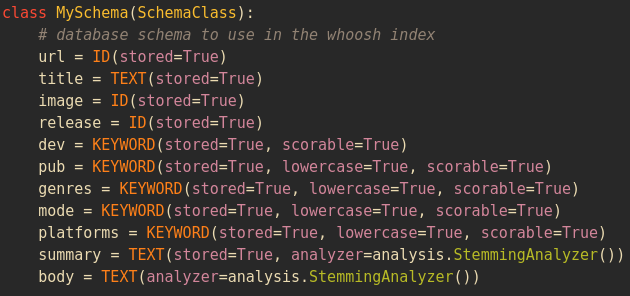
\includegraphics[width=3in]{whooshSchema}
\caption{Whoosh Schema}
\label{fig:whooshschema}
\end{figure}

In the above schema, attributes marked with ID are stored as the entire string. This is useful for the url, image, and release date as these attributes will not be searched over but they will need to be returned to the user. Attributes marked with KEYWORD are stored as each individual word in the string without any adjacency information to aid in matching queries. The attributes marked with TEXT store more information about the position of each word in the string to aid searches on these attributes. Anything with stored=True will be available to return to the user, but this will increase the size of the index. Since the body text will never be returned to the user there is no point in storing it. The option scorable=True allows the user to search over the keywords. The option lowercase=True converts all strings that are stored in the attribute to lowercase. For summary and body, we decided to use the default stemming analyzer in order to save space.

\section{Serving the data}
We are using the Flask module as an API to connect the backend to the frontend. The React frontend app will be able to request data through the API in order to display what the user wants. There are two API pages available for the frontend to request data:

/gameresults?[query string]

/searchresults?[query string]

The searchresults page has optional arguments for search, console, mode (disjunctive/conjunctive), and page number. The gameresults page is only expecting a title argument. Each argument in the query string is separated by a \& symbol.\\
Example: /searchresults?search=zombies\&console=xbox

The API utilizes these dynamic URLs to indicate the query and allow optional arguments. These URLs can be provided directly or created by the frontend. The data is provided in a JSON format. Only the relevant data for the API page is returned. The searchresult page returns the following JSON format:

\begin{minipage}[H]{\textwidth}
\begin{verbatim}
{
  "title": "Halo 3",
  "image": "cover art url",
  "url": "wiki article url",
  "console": "Xbox 360"
}
\end{verbatim}
\end{minipage}

The gameresult page returns the release date instead of the console information.

\section{Viewing the data}
The data will be displayed to the user using the React JavaScript library. React was chosen due to its high customizability and open source foundation, however in hindsight a library written in a more familiar language would have been a better choice. The styling of all elements is controlled by CSS files. 

\subsection{Design Choices}
A simple background, logo, and buttons were chosen to create a sleek home page. The search bar was created longer to fit six words, because the query will also search through the descriptions of the games. This allows the user to still find the game if they cannot remember the exact title. All fonts within the search bar and titles were chosen due to their clarity. 

In the search results page, the background is the same as the home page to create a continuous feel throughout the web app. The results are displayed in a grid 2 results wide and 5 results tall to fit 10 results per page. Each game shown has a slight shadow behing the box and the picture of the game to draw the users attention. While the mouse is hovering over the games title, it increases in size and is underlined. This is to give a responsive feel to the page while also making it easier for the user to read. 

In the game results page, each game is shown to the user horizontally. As the user scrolls a game off the screen, it increases in opacity and slides down to give an animated effect. When a game appears on the screen, it decreases in opacity and shifts up. This gives a responsive feel to the page. The timeline is also displayed horizontally below the games to give a continuous flow to the game results page. The white color in the timeline makes it pop, and draws the users eyes. 

\subsection{Functionality}
Each separate page and component displayed to the user is created in a separate javascript file. The users queries and search options are easily recorded and handled using state variables. These state variables make handling user requests easy, because as the state variable is updated the components shown to the user can be updated. UseEffect was used to run on the initial render for both the game results page and search results page. This is to fetch the data from the backend and display it to the user. UseEffect was also used in the search bar component to navigate to other pages whenever the user inputted a search. 

The data was requested from the backend using createSearchParams from 'react-router-dom'. This package allowed for the data to be requested at the same time as the front end navigated to the correct page. The package BrowserRouter was imported from 'react-router-dom' in order for the routes between the pages to be set. 

The color, fonts, and format are assigned in CSS files. Elements could be customized to hover, underlined, adjust size, change opacity, and rotated. Each page has a separate CSS file. 

\subsection{Citations}
Citations to articles

\section{Conclusions}
The front end of this project was not completed due to my lack of experience in javascript. We were able to import all data, but handling the data in javascript was the problem. The search results page is complete because there are only ten results displayed each page. However in the game results page, the timeline and the games have to be dynamically created due to the number of results returned varying. From the resources I could find, any solution offered did not allow me to dynamically set useState variables. This was also the case for the keywords in the advanced search menu. The overall structure of the front end is complete, without most of its features due to this problem. 
\end{document}  % This is where a 'short' article might terminate



%\appendix
%Appendix A
%\subsection{Introduction}
%\subsection{Collecting the data}
%\subsection{Indexing the data}
%\subsection{Serving the data}
%\subsection{Viewing the data}
%\subsection{Citations}
%\subsection{Conclusions}
%\subsection{References}